\documentclass{article}
% generated by Madoko, version 1.1.4
%mdk-data-line={1}


\usepackage[heading-base={2},section-num={False},bib-label={hide},fontspec={True}]{madoko2}
\usepackage[UTF8]{ctex}
\usepackage{geometry}
\usepackage{indentfirst}
%mdk-data-line={8}
\geometry{a4paper, left=3.18cm, right=3.18cm, top=2.54cm, bottom=2.54cm}
%mdk-data-line={9}
\setlength{\parindent}{0em}

\begin{document}



%mdk-data-line={20}
\mdxtitleblockstart{}
%mdk-data-line={20}
\mdxtitle{\mdline{20}MMORPG设计文档}%mdk
\mdxauthorstart{}
%mdk-data-line={25}
\mdxauthorname{\mdline{25}刘思尧 \& 苏宇皓}%mdk

%mdk-data-line={28}
\mdxauthoraddress{\mdline{28}BUPT}%mdk
\mdxauthorend\mdtitleauthorrunning{}{}\mdxtitleblockend%mdk
%mdk-begin-texraw
%mdk-data-line={23}
\newpage
\mdline{26}
\begin{mdtoc}%mdk

\section*{Contents}\label{sec-contents}%mdk%mdk

\begin{mdtocblock}%mdk

\mdtocitemx{1}{\mdref{1}{1.\hspace*{0.5em}项目介绍}}%mdk

\begin{mdtocblock}%mdk

\mdtocitemx{12}{\mdref{12}{1.1.\hspace*{0.5em}MMORPG}}%mdk

\mdtocitemx{13}{\mdref{13}{1.2.\hspace*{0.5em}运行机制}}%mdk
%mdk
\end{mdtocblock}%mdk

\mdtocitemx{2}{\mdref{2}{2.\hspace*{0.5em}游戏需求}}%mdk

\begin{mdtocblock}%mdk

\mdtocitemx{21}{\mdref{21}{2.1.\hspace*{0.5em}游戏流程}}%mdk

\mdtocitemx{22}{\mdref{22}{2.2.\hspace*{0.5em}名词解释}}%mdk

\mdtocitemx{23}{\mdref{23}{2.3.\hspace*{0.5em}游戏规则}}%mdk
%mdk
\end{mdtocblock}%mdk

\mdtocitemx{3}{\mdref{3}{3.\hspace*{0.5em}功能设计}}%mdk

\begin{mdtocblock}%mdk

\mdtocitemx{31}{\mdref{31}{3.1.\hspace*{0.5em}用户登陆、注册与创建角色}}%mdk

\mdtocitemx{32}{\mdref{32}{3.2.\hspace*{0.5em}角色交互}}%mdk

\mdtocitemx{33}{\mdref{33}{3.3.\hspace*{0.5em}购买与充值}}%mdk

\mdtocitemx{34}{\mdref{34}{3.4.\hspace*{0.5em}道具与装备}}%mdk

\mdtocitemx{35}{\mdref{35}{3.5.\hspace*{0.5em}副本与奖励}}%mdk

\mdtocitemx{36}{\mdref{36}{3.6.\hspace*{0.5em}多人联机}}%mdk
%mdk
\end{mdtocblock}%mdk

\mdtocitemx{4}{\mdref{4}{4.\hspace*{0.5em}数据库设计}}%mdk

\begin{mdtocblock}%mdk

\mdtocitemx{41}{\mdref{41}{4.1.\hspace*{0.5em}实体-关系模型}}%mdk

\mdtocitemx{42}{\mdref{42}{4.2.\hspace*{0.5em}数据库表结构}}%mdk

\mdtocitemx{43}{\mdref{43}{4.3.\hspace*{0.5em}数据库事务}}%mdk
%mdk
\end{mdtocblock}%mdk

\mdtocitemx{5}{\mdref{5}{5.\hspace*{0.5em}功能模块设计}}%mdk

\begin{mdtocblock}%mdk

\mdtocitemx{51}{\mdref{51}{5.1.\hspace*{0.5em}登陆模块}}%mdk

\mdtocitemx{52}{\mdref{52}{5.2.\hspace*{0.5em}玩家模块}}%mdk

\mdtocitemx{53}{\mdref{53}{5.3.\hspace*{0.5em}管理员模块}}%mdk

\mdtocitemx{54}{\mdref{54}{5.4.\hspace*{0.5em}队伍模块}}%mdk

\mdtocitemx{55}{\mdref{55}{5.5.\hspace*{0.5em}购物模块}}%mdk

\mdtocitemx{55.5}{\mdref{55.5}{5.6.\hspace*{0.5em}怪物模块}}%mdk

\mdtocitemx{56}{\mdref{56}{5.7.\hspace*{0.5em}副本模块}}%mdk

\mdtocitemx{57}{\mdref{57}{5.8.\hspace*{0.5em}充值模块}}%mdk

\mdtocitemx{58}{\mdref{58}{5.9.\hspace*{0.5em}物品迁移模块}}%mdk

\mdtocitemx{59}{\mdref{59}{5.10.\hspace*{0.5em}视图模块}}%mdk
%mdk
\end{mdtocblock}%mdk

\mdtocitemx{6}{\mdref{6}{6.\hspace*{0.5em}技术和环境分析}}%mdk

\begin{mdtocblock}%mdk

\mdtocitemx{61}{\mdref{61}{6.1.\hspace*{0.5em}开发技术}}%mdk

\mdtocitemx{62}{\mdref{62}{6.2.\hspace*{0.5em}开发环境}}%mdk

\mdtocitemx{63}{\mdref{63}{6.3.\hspace*{0.5em}生产环境}}%mdk
%mdk
\end{mdtocblock}%mdk
%mdk
\end{mdtocblock}%mdk
%mdk
\end{mdtoc}%mdk
%mdk-begin-texraw
%mdk-data-line={29}
\newpage

%mdk-data-line={32}
\section{\mdline{32}1.\hspace*{0.5em}\mdline{32}项目介绍}\label{1}%mdk%mdk

%mdk-data-line={34}
\subsection{\mdline{34}1.1.\hspace*{0.5em}\mdline{34}MMORPG}\label{12}%mdk%mdk

%mdk-data-line={36}
\noindent\mdline{36}MMORPG ,是英文 Massive (或 Massively ) Multiplayer Online Role-Playing Game的缩写。至今尚未有\mdline{36}~\href{https://baike.baidu.com/item/MMORPG}{MMORPG}\mdline{36} 的正式中文译名,而在中国比较常见的译法则是\mdline{36}\textquotedblleft{}大型多人在线角色扮演游戏\textquotedblright{}\mdline{36},是网络游戏的一种。在所有角色扮演游戏中,玩家都要扮演一个虚构角色,并控制该角色的许多活动。%mdk

%mdk-data-line={38}
\subsection{\mdline{38}1.2.\hspace*{0.5em}\mdline{38}运行机制}\label{13}%mdk%mdk

%mdk-data-line={40}
\noindent\mdline{40}MMORPG分为客户端和服务器两部分。我们使用浏览器作为客户端。玩家从客户端通过互联网连接,登陆服务器端后才能进行游戏。%mdk

%mdk-data-line={42}
\mdline{42}玩家的资料保存在服务器端。游戏的过程,是玩家扮演的角色和其他玩家控制的角色在网络虚拟空间中实时互动。而非玩家扮演的角色(即NPC)则往往是在游戏中提供特殊服务的人物,如销售虚拟物品,提供任务等。%mdk

%mdk-data-line={44}
\mdline{44}我们提供服务器供玩家游戏,负责管理游戏中的虚拟世界,并不断为游戏做出更新,以便留住玩家以及吸引其他人来玩这款游戏。%mdk

%mdk-data-line={46}
\section{\mdline{46}2.\hspace*{0.5em}\mdline{46}游戏需求}\label{2}%mdk%mdk

%mdk-data-line={48}
\subsection{\mdline{48}2.1.\hspace*{0.5em}\mdline{48}游戏流程}\label{21}%mdk%mdk

%mdk-data-line={50}
\noindent\mdline{50}每一个\mdline{50}\textbf{用户}\mdline{50}创建自己的\mdline{50}\textbf{角色}\mdline{50}。系统内置了\mdline{50}\textbf{怪物}\mdline{50},角色可以\mdline{50}\textbf{组队}\mdline{50}进入\mdline{50}\textbf{副本}\mdline{50}攻击\mdline{50}\textbf{怪物}\mdline{50}获得各种奖励。 角色还可以在地图上的\mdline{50}\textbf{商店}\mdline{50}购物,相互添加\mdline{50}\textbf{好友}\mdline{50}。\mdline{50}\textbf{队伍}\mdline{50}之间可以发起对战。%mdk

%mdk-data-line={52}
\subsection{\mdline{52}2.2.\hspace*{0.5em}\mdline{52}名词解释}\label{22}%mdk%mdk

%mdk-data-line={54}
\noindent\mdline{54}\textbf{角色}\mdline{54}: 角色是玩家进行游戏的载体,玩家操控角色在游戏中行动。 角色拥有一系列属性,包括昵称、生命值(HP)、攻击力、防御力、经验值、金钱。%mdk

%mdk-data-line={56}
\mdline{56}\textbf{好友}\mdline{56}: 好友是两个角色之间的对等关系,互为好友的两个角色可以更快的找到对方。%mdk

%mdk-data-line={58}
\mdline{58}\textbf{仓库}\mdline{58}: 一个角色拥有多个仓库,仓库中可以存储角色的物品(包括装备和道具)。 角色在攻打副本时不可以访问仓库。%mdk

%mdk-data-line={60}
\mdline{60}\textbf{背包}\mdline{60}: 一个角色有且只有一个背包,用于在攻打副本时携带所需物品。%mdk

%mdk-data-line={62}
\mdline{62}\textbf{道具}\mdline{62}: 道具是能够在一次攻打副本期间对玩家某项数值进行增强的物品。%mdk

%mdk-data-line={64}
\mdline{64}\textbf{装备}\mdline{64}: 装备分为剑、盾、铠甲三种,可以提升角色的部分属性值。角色不能装备一件以上的同种装备。%mdk

%mdk-data-line={66}
\mdline{66}\textbf{宠物}\mdline{66}: 角色可以饲养宠物(从商店购买),宠物会跟随在玩家身后,但只有装饰作用。%mdk

%mdk-data-line={68}
\mdline{68}\textbf{队伍}\mdline{68}: 一支队伍由一个或更多玩家组成,并有一个队长。队伍可以攻打副本。%mdk

%mdk-data-line={70}
\mdline{70}\textbf{副本}\mdline{70}: 副本是一张地图。副本中有怪物,角色可以在副本中攻击怪物并得到奖励。%mdk

%mdk-data-line={72}
\mdline{72}\textbf{主世界}\mdline{72}: 主世界是一张地图。角色可以在主世界访问商店、仓库或进入副本。%mdk

%mdk-data-line={74}
\mdline{74}\textbf{地图}\mdline{74}: 地图是一个二维矩阵,每一格被分配了地形。角色可以在地图中移动并触发事件。%mdk

%mdk-data-line={76}
\mdline{76}\textbf{金币}\mdline{76}: 游戏中的虚拟货币。%mdk

%mdk-data-line={78}
\subsection{\mdline{78}2.3.\hspace*{0.5em}\mdline{78}游戏规则}\label{23}%mdk%mdk

%mdk-data-line={80}
\subsubsection{\mdline{80}2.3.1.\hspace*{0.5em}\mdline{80}用户与角色}\label{231}%mdk%mdk

%mdk-data-line={82}
\noindent\mdline{82}用户登录后,可以选择创建角色,如果已有角色,可以销毁角色或使用该角色进入游戏。%mdk

%mdk-data-line={84}
\mdline{84}角色有三个装备槽——剑、盾、铠甲。每个槽只能装备一件装备。%mdk

%mdk-data-line={86}
\mdline{86}角色可以申请与其他角色结为好友,若对方同意,则将对方加入双方的好友列表。%mdk

%mdk-data-line={88}
\subsubsection{\mdline{88}2.3.2.\hspace*{0.5em}\mdline{88}主世界}\label{232}%mdk%mdk

%mdk-data-line={90}
\noindent\mdline{90}所有在线玩家位于主地图或副本地图。 角色进入游戏后,出生于主地图随机位置。%mdk

%mdk-data-line={92}
\mdline{92}角色可以通过商店购买/出售可交易物品,可交易物品包括所有装备、道具、宠物。%mdk

%mdk-data-line={94}
\mdline{94}角色可以通过副本入口点进入对应的副本。%mdk

%mdk-data-line={96}
\mdline{96}道具可以在仓库与背包之间转移。%mdk

%mdk-data-line={98}
\mdline{98}用户可以通过界面内菜单进行人民币充值,1元=100金币。%mdk

%mdk-data-line={100}
\subsubsection{\mdline{100}2.3.3.\hspace*{0.5em}\mdline{100}副本}\label{233}%mdk%mdk

%mdk-data-line={102}
\noindent\mdline{102}怪物在且仅在副本中出现。 角色尝试进入怪物所在格子时视为发动攻击,参照战斗规则。 如果怪兽在战斗中死亡,会在自己周围 3\mdline{102}*\mdline{102}3 的方格内掉落物品,包括装备与道具。%mdk

%mdk-data-line={104}
\mdline{104}战斗规则:%mdk

%mdk-data-line={106}
\begin{enumerate}[noitemsep,topsep=\mdcompacttopsep]%mdk

%mdk-data-line={106}
\item\mdline{106}发起战斗的一方先进行攻击,令攻击方为A,防御方为B。%mdk

%mdk-data-line={107}
\item\mdline{107}每次攻击, A 对 B 的 HP 造成 A攻击\mdline{107} \mdline{107}- B防御 点伤害。%mdk

%mdk-data-line={108}
\item\mdline{108}一次攻击结束后,攻击与防御方交换,进行下一轮攻击。%mdk

%mdk-data-line={109}
\item\mdline{109}有一方的 HP 小于等于 0 时,战斗结束。%mdk
%mdk
\end{enumerate}%mdk

%mdk-data-line={111}
\noindent\mdline{111}角色可以在非战斗时刻使用道具。%mdk

%mdk-data-line={114}
\section{\mdline{114}3.\hspace*{0.5em}\mdline{114}功能设计}\label{3}%mdk%mdk

%mdk-data-line={116}
\noindent\mdline{116}下面是根据上文给出的需求分析得到的软件功能要求。%mdk

%mdk-data-line={118}
\subsection{\mdline{118}3.1.\hspace*{0.5em}\mdline{118}用户登陆、注册与创建角色}\label{31}%mdk%mdk

%mdk-data-line={120}
\subsubsection{\mdline{120}3.1.1.\hspace*{0.5em}\mdline{120}用户登录注册}\label{311}%mdk%mdk

%mdk-data-line={122}
\noindent\mdline{122}登录注册页面前端部分内容,主要是用户账号和密码在js代码里做对应的正则匹配,这是验证的第一步,保证用户输入格式的正确性同时也从一方面减少用户向后台发送没必要的错误请求。前端向后端请求的方式使用POST。 在后台接收前端传送的信息同样要经过验证正则的规则匹配步骤,因为有可能一些人并不是通过合法的方式进行访问,可以减少没必要的数据库查询。%mdk

%mdk-data-line={124}
\subsubsection{\mdline{124}3.1.2.\hspace*{0.5em}\mdline{124}用户密码安全性}\label{312}%mdk%mdk

%mdk-data-line={126}
\noindent\mdline{126}由于很多人习惯使用相同的密码,为了降低撞库的风险,不应当使用明文存储密码。 密码的保存使用“密钥\mdline{126} \mdline{126}+ 不可逆加密算”,使用如 sha1,sha256 等不可逆的加密算法进行加密后再存入数据库。%mdk

%mdk-data-line={128}
\subsubsection{\mdline{128}3.1.3.\hspace*{0.5em}\mdline{128}登录状态的保存}\label{313}%mdk%mdk

%mdk-data-line={130}
\noindent\mdline{130}由于http协议是无状态的,所以用户的登录状态就要靠后台相应的数据来记录,用户登录成功后在 seesion 中保存登录用户,然后将该状态通过 cookie 返回到客户端,之后通过比对 cookie 和 seesion 信息来验证用户是否已登录。%mdk

%mdk-data-line={132}
\subsubsection{\mdline{132}3.1.4.\hspace*{0.5em}\mdline{132}密码找回功能}\label{314}%mdk%mdk

%mdk-data-line={134}
\noindent\mdline{134}因为后台密码是加密的,无法提供明文密码的找回。 但是可以通过手机短信验证或者邮箱验证,验证成功后直接设置新密码。 安全起见,向重置密码的 url 地址加入时间戳和唯一随机数来保证这个链接只在某个时间内有效,如果在密码修改成功或者事件过期,就把这个唯一随机数给删除,保存密码方式同上。%mdk

%mdk-data-line={136}
\subsubsection{\mdline{136}3.1.5.\hspace*{0.5em}\mdline{136}角色的创建}\label{315}%mdk%mdk

%mdk-data-line={138}
\noindent\mdline{138}一个用户只能创建一名角色,而且没有角色的用户无法进行游戏。 因此可以让用户在创建账号后立即进行角色的创建。 在前端让用户挑选自己喜欢的皮肤与特性等角色属性,将数据传给后端存入数据库。 角色创建后直接进入游戏。 一般不希望用户经常修改角色,因此将删除角色的功能放在进入游戏后的设置界面内。%mdk

%mdk-data-line={140}
\begin{figure}[tbp]%mdk
\begin{mdcenter}%mdk

%mdk-data-line={141}
\noindent\mdline{141}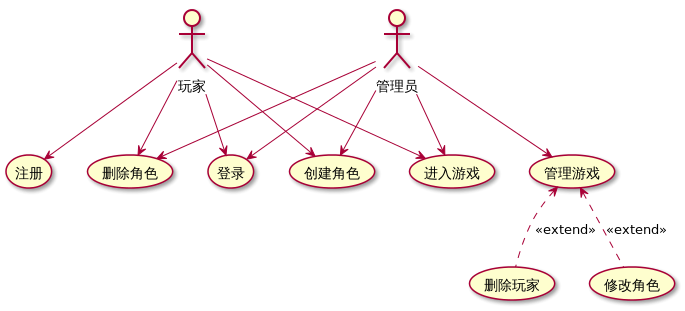
\includegraphics[keepaspectratio=true,width=\dimwidth{1.00}]{./img/1}{}\mdline{141}%mdk

%mdk-data-line={142}
\mdhr{}%mdk

%mdk-data-line={143}
\noindent\mdline{143}\mdcaption{\textbf{Figure~\mdcaptionlabel{1}.}~\mdcaptiontext{用例图}}%mdk
%mdk
\end{mdcenter}%mdk
\end{figure}%mdk

%mdk-data-line={144}
\begin{figure}[tbp]%mdk
\begin{mdcenter}%mdk

%mdk-data-line={145}
\noindent\mdline{145}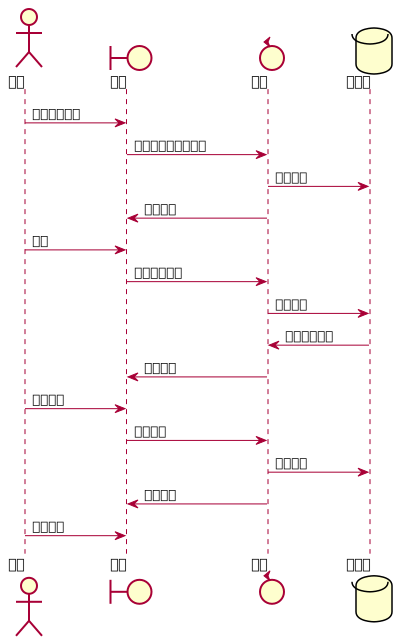
\includegraphics[keepaspectratio=true,width=\dimwidth{0.70}]{./img/7}{}\mdline{145}%mdk

%mdk-data-line={146}
\mdhr{}%mdk

%mdk-data-line={147}
\noindent\mdline{147}\mdcaption{\textbf{Figure~\mdcaptionlabel{2}.}~\mdcaptiontext{主流程时序图}}%mdk
%mdk
\end{mdcenter}%mdk
\end{figure}%mdk

%mdk-data-line={148}
\subsection{\mdline{148}3.2.\hspace*{0.5em}\mdline{148}角色交互}\label{32}%mdk%mdk

%mdk-data-line={150}
\subsubsection{\mdline{150}3.2.1.\hspace*{0.5em}\mdline{150}导航与事件触发}\label{321}%mdk%mdk

%mdk-data-line={152}
\noindent\mdline{152}秉承简单的原则,基本只使用上下左右四个按钮。 玩家通过上下左右在地图上移动,如果玩家尝试进入某个特殊的格子(例如怪兽所在的格子、商店所在的格子),就触发事件。 可以触发的事件包括:%mdk

%mdk-data-line={154}
\begin{itemize}[noitemsep,topsep=\mdcompacttopsep]%mdk

%mdk-data-line={154}
\item\mdline{154}与怪兽战斗%mdk

%mdk-data-line={155}
\item\mdline{155}打开商店界面%mdk

%mdk-data-line={156}
\item\mdline{156}打开仓库界面%mdk

%mdk-data-line={157}
\item\mdline{157}进入副本%mdk

%mdk-data-line={158}
\item\mdline{158}拾取物品%mdk

%mdk-data-line={159}
\item\mdline{159}离开副本%mdk
%mdk
\end{itemize}%mdk

%mdk-data-line={161}
\subsubsection{\mdline{161}3.2.2.\hspace*{0.5em}\mdline{161}其他操作}\label{322}%mdk%mdk

%mdk-data-line={163}
\noindent\mdline{163}出去导航时出发的时间,角色还能进行许多其他操作,通过前端 UI 引导,使用鼠标完成。 这些操作主要与其他玩家交互、道具与装备的使用与转移、在商店购买有关。 这些操作会在后面详细说明。%mdk

%mdk-data-line={165}
\begin{figure}[tbp]%mdk
\begin{mdcenter}%mdk

%mdk-data-line={166}
\noindent\mdline{166}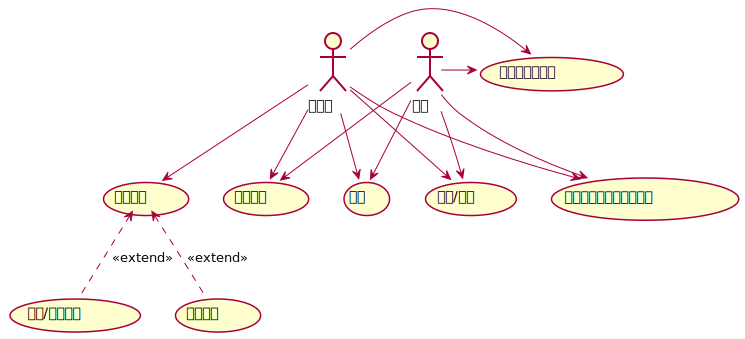
\includegraphics[keepaspectratio=true,width=\dimwidth{1.00}]{./img/2}{}\mdline{166}%mdk

%mdk-data-line={167}
\mdhr{}%mdk

%mdk-data-line={168}
\noindent\mdline{168}\mdcaption{\textbf{Figure~\mdcaptionlabel{3}.}~\mdcaptiontext{用例图}}%mdk
%mdk
\end{mdcenter}%mdk
\end{figure}%mdk

%mdk-data-line={169}
\subsection{\mdline{169}3.3.\hspace*{0.5em}\mdline{169}购买与充值}\label{33}%mdk%mdk

%mdk-data-line={171}
\subsubsection{\mdline{171}3.3.1.\hspace*{0.5em}\mdline{171}商店购物}\label{331}%mdk%mdk

%mdk-data-line={173}
\noindent\mdline{173}游戏中的虚拟货币称为金币。 玩家通过导航进入商店后,会弹出商店菜单。 游戏设定为在商店中可以无限量购买或出售所有的物品,包括宠物、装备与道具。 因此不必存储商店中的库存余量。 前端需要按照分类展示所有的物品,玩家根据需要将要购买的物品加入购物清单,清单在加入第一个物品时自动生成。 清单显示在一个单独的窗口中,并实时计算当前所有物品的金币数。 在玩家选择完毕后,可以进行结算,从玩家余额中扣除相应的金币,并向玩家对应的仓库中添加所购买的物品,这是前端与后端进行数据传递的一步。%mdk

%mdk-data-line={175}
\subsubsection{\mdline{175}3.3.2.\hspace*{0.5em}\mdline{175}人民币充值}\label{332}%mdk%mdk

%mdk-data-line={177}
\noindent\mdline{177}玩家获取金币有两种途径,一是攻打副本时怪物掉落以及副本奖励,一是通过人民币充值。 由于涉及到金钱交易,处理需要十分谨慎,在后端采用数据库事务模式。 与各种支付平台对接,使得用户可以通过多种方式支付。%mdk

%mdk-data-line={179}
\begin{figure}[tbp]%mdk
\begin{mdcenter}%mdk

%mdk-data-line={180}
\noindent\mdline{180}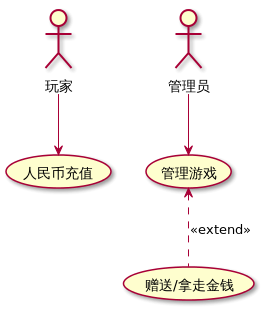
\includegraphics[keepaspectratio=true,width=\dimwidth{0.50}]{./img/3}{}\mdline{180}%mdk

%mdk-data-line={181}
\mdhr{}%mdk

%mdk-data-line={182}
\noindent\mdline{182}\mdcaption{\textbf{Figure~\mdcaptionlabel{4}.}~\mdcaptiontext{用例图}}%mdk
%mdk
\end{mdcenter}%mdk
\end{figure}%mdk

%mdk-data-line={183}
\begin{figure}[tbp]%mdk
\begin{mdcenter}%mdk

%mdk-data-line={184}
\noindent\mdline{184}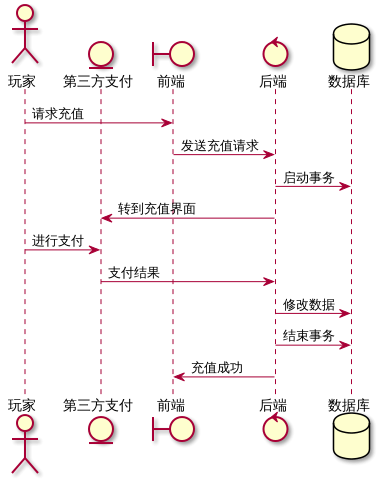
\includegraphics[keepaspectratio=true,width=\dimwidth{0.70}]{./img/9}{}\mdline{184}%mdk

%mdk-data-line={185}
\mdhr{}%mdk

%mdk-data-line={186}
\noindent\mdline{186}\mdcaption{\textbf{Figure~\mdcaptionlabel{5}.}~\mdcaptiontext{充值时序图}}%mdk
%mdk
\end{mdcenter}%mdk
\end{figure}%mdk

%mdk-data-line={187}
\subsection{\mdline{187}3.4.\hspace*{0.5em}\mdline{187}道具与装备}\label{34}%mdk%mdk

%mdk-data-line={189}
\noindent\mdline{189}设计道具与装备是为了丰富游戏内容,增强玩家的体验。%mdk

%mdk-data-line={191}
\mdline{191}道具用于在副本中使用,增加玩家的生命值或攻击力。 玩家有两个容器可以存储道具:仓库与背包。 玩家的所有道具都可以存储在仓库中,但是在副本中无法访问仓库,要将道具放入背包(可容纳的数量有限)带入副本才可以使用。 因此要设计两个展示界面:仓库与背包,仓库在主界面通过导航事件访问,背包可以在游戏界面下方的状态栏打开。 玩家在仓库界面时可以浏览自己拥有的所有道具,也可以在仓库和背包之间转移物品。 在攻打副本时,可以打开背包并使用其中的道具。 同时,在攻打副本过程中获得的战利品也会被放入背包。%mdk

%mdk-data-line={193}
\mdline{193}装备可以提升玩家的属性,分为剑、盾、铠甲三类。 玩家同一时间只能装备一把剑、一面盾和一身铠甲。 装备只能放置在仓库中,如果在副本中获得了装备会被传送到仓库。 玩家可以在浏览仓库时选择某件装备并穿上。%mdk

%mdk-data-line={195}
\mdline{195}仓库分为装备仓库和道具仓库两种,玩家可以自行创建新的仓库(为了方便对物品进行分类)。%mdk

%mdk-data-line={197}
\begin{figure}[tbp]%mdk
\begin{mdcenter}%mdk

%mdk-data-line={198}
\noindent\mdline{198}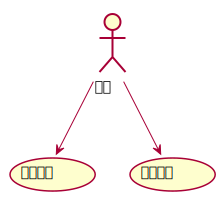
\includegraphics[keepaspectratio=true,width=\dimwidth{0.30}]{./img/4}{}\mdline{198}%mdk

%mdk-data-line={199}
\mdhr{}%mdk

%mdk-data-line={200}
\noindent\mdline{200}\mdcaption{\textbf{Figure~\mdcaptionlabel{6}.}~\mdcaptiontext{用例图}}%mdk
%mdk
\end{mdcenter}%mdk
\end{figure}%mdk

%mdk-data-line={201}
\subsection{\mdline{201}3.5.\hspace*{0.5em}\mdline{201}副本与奖励}\label{35}%mdk%mdk

%mdk-data-line={203}
\noindent\mdline{203}玩家可以攻打副本并获得奖励,这也是用户玩游戏的主要动机。 怪兽只出现在副本中,玩家可以在主世界内与其它玩家组队并攻打副本,通过杀死副本内的怪兽来得到奖励。 按照设定,副本指某一个特定的含有怪物的地图。 副本对每一个队伍是独立的,也就是说一支队伍攻打副本并不会对队伍以外的玩家造成任何影响。 副本和主世界一样,都是一张地图,因此采用与主世界相同的显示模块,但是增加了触发战斗的导航事件。%mdk

%mdk-data-line={205}
\mdline{205}队伍进入副本所在位置便可以攻打副本,这时从数据库查询对应副本的地图并返回给前端,前端通过后端同步其它在线玩家的位置信息,并在拾取战利品时修改数据库。%mdk

%mdk-data-line={207}
\begin{figure}[tbp]%mdk
\begin{mdcenter}%mdk

%mdk-data-line={208}
\noindent\mdline{208}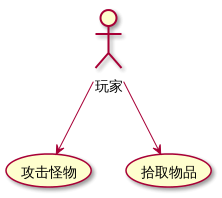
\includegraphics[keepaspectratio=true,width=\dimwidth{0.30}]{./img/5}{}\mdline{208}%mdk

%mdk-data-line={209}
\mdhr{}%mdk

%mdk-data-line={210}
\noindent\mdline{210}\mdcaption{\textbf{Figure~\mdcaptionlabel{7}.}~\mdcaptiontext{用例图}}%mdk
%mdk
\end{mdcenter}%mdk
\end{figure}%mdk

%mdk-data-line={211}
\subsection{\mdline{211}3.6.\hspace*{0.5em}\mdline{211}多人联机}\label{36}%mdk%mdk

%mdk-data-line={213}
\noindent\mdline{213}进行多人联机需要获取所有其他玩家的状态(位置、朝向、动作等),这样的同步通过在后端记录在线玩家的状态完成。 这些状态并不需要被存入数据库,因为没有持久化的必要。 前端每隔一定时间就与后端进行同步,来更新所有玩家的状态。%mdk

%mdk-data-line={215}
\mdline{215}除了在地图上显示所有在线玩家,还有与其他玩家互动的需求。 为此,设置一个消息箱,玩家 A 希望与玩家 B 组队或结为好友时,可以发送消息,玩家 B 看到消息后即可做出应答。%mdk

%mdk-data-line={217}
\begin{figure}[tbp]%mdk
\begin{mdcenter}%mdk

%mdk-data-line={218}
\noindent\mdline{218}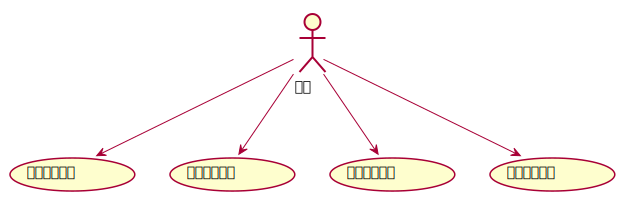
\includegraphics[keepaspectratio=true,width=\dimwidth{0.90}]{./img/6}{}\mdline{218}%mdk

%mdk-data-line={219}
\mdhr{}%mdk

%mdk-data-line={220}
\noindent\mdline{220}\mdcaption{\textbf{Figure~\mdcaptionlabel{8}.}~\mdcaptiontext{用例图}}%mdk
%mdk
\end{mdcenter}%mdk
\end{figure}%mdk

%mdk-data-line={221}
\begin{figure}[tbp]%mdk
\begin{mdcenter}%mdk

%mdk-data-line={222}
\noindent\mdline{222}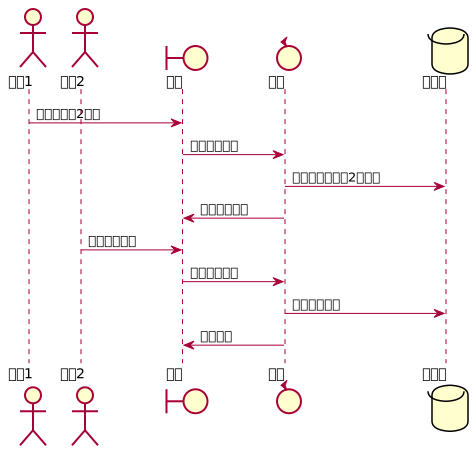
\includegraphics[keepaspectratio=true,width=\dimwidth{0.75}]{./img/8}{}\mdline{222}%mdk

%mdk-data-line={223}
\mdhr{}%mdk

%mdk-data-line={224}
\noindent\mdline{224}\mdcaption{\textbf{Figure~\mdcaptionlabel{9}.}~\mdcaptiontext{组队时序图}}%mdk
%mdk
\end{mdcenter}%mdk
\end{figure}%mdk

%mdk-data-line={226}
\section{\mdline{226}4.\hspace*{0.5em}\mdline{226}数据库设计}\label{4}%mdk%mdk

%mdk-data-line={228}
\subsection{\mdline{228}4.1.\hspace*{0.5em}\mdline{228}实体-关系模型}\label{41}%mdk%mdk

%mdk-data-line={230}
\begin{figure}[tbp]%mdk
\begin{mdcenter}%mdk

%mdk-data-line={231}
\noindent\mdline{231}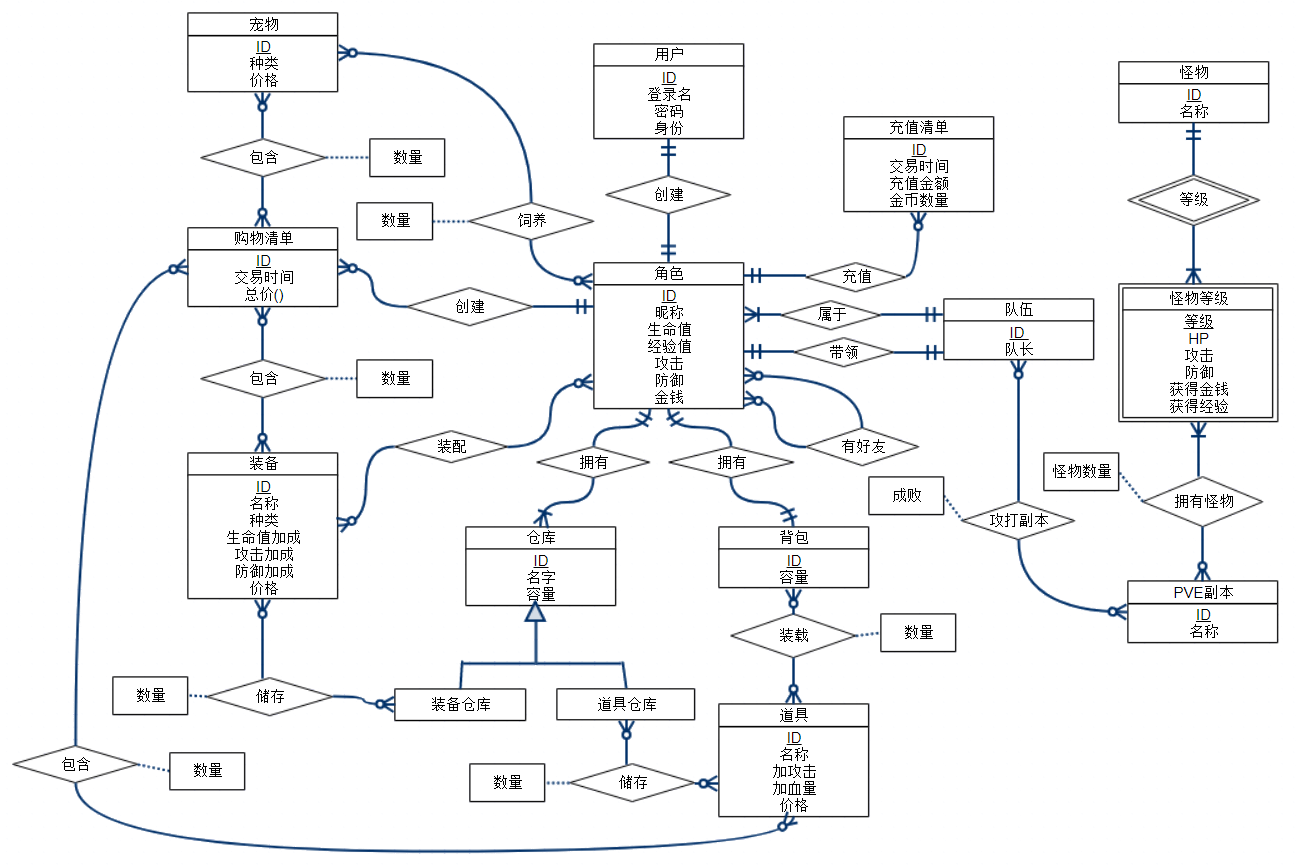
\includegraphics[keepaspectratio=true,width=\dimwidth{1.00}]{./erd}{}\mdline{231}%mdk

%mdk-data-line={232}
\mdhr{}%mdk

%mdk-data-line={233}
\noindent\mdline{233}\mdcaption{\textbf{Figure~\mdcaptionlabel{10}.}~\mdcaptiontext{E-R图}}%mdk
%mdk
\end{mdcenter}%mdk
\end{figure}%mdk

%mdk-data-line={234}
\subsubsection{\mdline{234}4.1.1.\hspace*{0.5em}\mdline{234}ER模型说明}\label{411}%mdk%mdk

%mdk-data-line={236}
\noindent\mdline{236}用户-角色:一个用户能且仅能创建一个角色,用户用作登陆和账号管理,角色再游戏中使用,他们是一一对应、双方全参与关系。%mdk

%mdk-data-line={238}
\mdline{238}角色-充值清单:一个角色可以没有账单或多个账单,但每一个账单必须要有一个角色与之对应,角色-账单为一对多关系,账单全参与。%mdk

%mdk-data-line={240}
\mdline{240}角色-队伍:一个角色属于且仅属于一支队伍,一个队伍至少有一个角色,因此角色、队伍均为全参与,角色-队伍为多对一。%mdk

%mdk-data-line={242}
\mdline{242}队伍-PVE副本:一个队伍可以攻打多个副本,一个副本可以由多个队伍攻打,均为部分参与,队伍-副本为一对多。%mdk

%mdk-data-line={244}
\mdline{244}PVE副本-怪物等级:一个副本中有1个到多个怪物,每个怪物可以在0个或多个副本中,副本全参与,多对多关系。%mdk

%mdk-data-line={246}
\mdline{246}怪物等级-怪物:怪物等级为弱实体集合,表示不同等级的同种怪物,怪物id和其等级共同缺点一只怪物。双方全参与,为多对一关系。%mdk

%mdk-data-line={248}
\mdline{248}角色-背包:一个角色有且仅有一个背包,一个背包也只由一个人拥有,双方全参与,为一对一关系。%mdk

%mdk-data-line={250}
\mdline{250}背包-道具:一个背包可以装配有0个或多个道具,一种道具可以在0个或多个背包中。都是部分参与,为多对多关系。%mdk

%mdk-data-line={252}
\mdline{252}角色-仓库:一个角色拥有若干仓库(仓库分为装备仓库和道具仓库),一个仓库只能由一个角色拥有,双方全参与,为一对一多关系。%mdk

%mdk-data-line={254}
\mdline{254}道具仓库-道具:一个道具仓库可以储存有0个或多个道具,一种道具可以在0个或多个道具仓库中。都是部分参与,为多对多关系。%mdk

%mdk-data-line={256}
\mdline{256}装备仓库-装备:一个装备仓库可以储存有0个或多个装备,一种装备可以在0个或多个装备仓库中。都是部分参与,为多对多关系。%mdk

%mdk-data-line={258}
\mdline{258}角色-装备:一个角色可以装配0个或多个装备,一种装备可以在0个或多个装备仓库中。都是部分参与,为多对多关系。%mdk

%mdk-data-line={260}
\mdline{260}角色-购物清单:一个角色可以有0个或多个购物清单,一个购物清单可以只能一个角色拥有,一个购物清单必须对应一个角色。角色部分参与,购物清单全参与,为一对多关系。%mdk

%mdk-data-line={262}
\mdline{262}角色-宠物:一个角色可以饲养若干个宠物,每种宠物可以有若干个饲养者。双方都是部分参与,为多对多关系。%mdk

%mdk-data-line={264}
\mdline{264}购物清单-宠物/装备/道具:一个宠物清单中可以有多个各种宠物/装备/道具,一种宠物/装备/道具可以在多个清单中。%mdk

%mdk-data-line={266}
\subsection{\mdline{266}4.2.\hspace*{0.5em}\mdline{266}数据库表结构}\label{42}%mdk%mdk

%mdk-data-line={268}
\noindent\mdline{268}\textbf{用户}\mdline{268}:%mdk
\begin{mdpre}%mdk
\noindent User(user\_id,~name,~password,~identity,~phone\_num,\\
\preindent{5}email,~verify\_code,~expire\_time);`%mdk
\end{mdpre}
%mdk-data-line={275}
\mdhr{}%mdk

%mdk-data-line={277}
\noindent\mdline{277}由于\mdline{277}\textbf{用户}\mdline{277}和\mdline{277}\textbf{角色}\mdline{277}有一一对应关系,用户为主表,在角色中创建外键user\mdline{277}\_\mdline{277}id。因为一一对应,外键为\mdline{277}\textbf{unique}\mdline{277};因为全参与,外键为\mdline{277}\textbf{not null}\mdline{277}。%mdk

%mdk-data-line={279}
\mdline{279}一个角色至少在一个\mdline{279}\textbf{队伍}\mdline{279}里,一个队伍可以有多个人,在角色中创建外键team\mdline{279}\_\mdline{279}id,外键为\mdline{279}\textbf{unique}\mdline{279};因为全参与,外键为\mdline{279}\textbf{not null}\mdline{279}。%mdk

%mdk-data-line={281}
\mdline{281}\textbf{角色}\mdline{281}:%mdk
\begin{mdpre}%mdk
\noindent Role(role\_id,~nickname,~hp,~exp,~atk,~def,\\
\preindent{5}money,~user\_id,~team\_id);%mdk
\end{mdpre}
%mdk-data-line={288}
\mdhr{}%mdk

%mdk-data-line={290}
\noindent\mdline{290}\textbf{仓库}\mdline{290}和角色为多对一,在仓库中创建外键role\mdline{290}\_\mdline{290}id。因为全参与,外键为\mdline{290}\textbf{not null}\mdline{290}:%mdk
\begin{mdpre}%mdk
\noindent EquipRepository(rep\_id,~name,~volume,~role\_id);\\
ItemRepository(rep\_id,~name,~volume,~role\_id);%mdk
\end{mdpre}
%mdk-data-line={297}
\mdhr{}%mdk

%mdk-data-line={299}
\noindent\mdline{299}\textbf{背包}\mdline{299}和角色为多对一,在背包中创建外键role\mdline{299}\_\mdline{299}id。因为全参与,外键为\mdline{299}\textbf{not null}\mdline{299}:%mdk

%mdk-data-line={301}
\mdline{301}\mdcode{Backpack(backpack\_id,~name,~volume,~role\_id);}\mdline{301}%mdk

%mdk-data-line={303}
\mdhr{}%mdk

%mdk-data-line={305}
\noindent\mdline{305}\textbf{充值清单}\mdline{305}和角色为多对一,在账单中创建外键role\mdline{305}\_\mdline{305}id。因为全参与,外键为\mdline{305}\textbf{not null}\mdline{305}:%mdk

%mdk-data-line={307}
\mdline{307}\mdcode{Bill(bill\_id,~time,~deposit,~money,~role\_id);}\mdline{307}%mdk

%mdk-data-line={309}
\mdline{309}一个\mdline{309}\textbf{队伍}\mdline{309}有一个队长,建立外键leader。因为一一对应,外键为\mdline{309}\textbf{unique}\mdline{309};因为全参与,外键为\mdline{309}\textbf{not null}\mdline{309}:%mdk

%mdk-data-line={311}
\mdline{311}\mdcode{Team(team\_id,~leader);}\mdline{311}%mdk

%mdk-data-line={313}
\mdhr{}%mdk

%mdk-data-line={315}
\noindent\mdline{315}\textbf{副本}\mdline{315}: \mdline{315}\mdcode{Dungeons(dungeons\_id,~name);}\mdline{315}%mdk

%mdk-data-line={317}
\mdhr{}%mdk

%mdk-data-line={319}
\noindent\mdline{319}\textbf{副本}\mdline{319}和\mdline{319}\textbf{队伍}\mdline{319}是多对多关系,因此创建一张新表,主键为team\mdline{319}\_\mdline{319}id和role\mdline{319}\_\mdline{319}id:%mdk

%mdk-data-line={321}
\mdline{321}\mdcode{Fights(team\_id,~dungeons\_id,~result);}\mdline{321}%mdk

%mdk-data-line={323}
\mdhr{}%mdk

%mdk-data-line={325}
\noindent\mdline{325}\textbf{怪物}\mdline{325}: \mdline{325}\mdcode{Monster(monster\_id,name);}\mdline{325}%mdk

%mdk-data-line={327}
\mdline{327}\textbf{怪物的等级}\mdline{327}是弱实体,需要怪物加上其等级才能作为一个实体,因此monster\mdline{327}\_\mdline{327}id和level共同作为主键:%mdk

%mdk-data-line={329}
\mdline{329}\mdcode{MonsterLevel(monster\_id,~level,~hp,~atk,~def,~money,~exp);}\mdline{329}%mdk

%mdk-data-line={331}
\mdhr{}%mdk

%mdk-data-line={333}
\noindent\mdline{333}\textbf{副本和怪物}\mdline{333}实体是多对多关系,因此创建一张新表:%mdk

%mdk-data-line={335}
\mdline{335}\mdcode{HaveMonster(dungeon\_id,monster\_id,max\_num);}\mdline{335}%mdk

%mdk-data-line={337}
\mdhr{}%mdk

%mdk-data-line={339}
\noindent\mdline{339}\textbf{道具}\mdline{339}: \mdline{339}\mdcode{Item(item\_id,~name,~kind,~hp,~atk,~def,~price);}\mdline{339}%mdk

%mdk-data-line={341}
\mdhr{}%mdk

%mdk-data-line={343}
\noindent\mdline{343}\textbf{装备}\mdline{343}: \mdline{343}\mdcode{Equipment(equip\_id,~name,~hp,~atk,~price);}\mdline{343}%mdk

%mdk-data-line={345}
\mdhr{}%mdk

%mdk-data-line={347}
\noindent\mdline{347}\textbf{装备和仓库}\mdline{347}是多对多关系,因此创建一张新表:%mdk

%mdk-data-line={349}
\mdline{349}\mdcode{StoreEquipment(rep\_id,~eqiup\_id,~number);}\mdline{349}%mdk

%mdk-data-line={351}
\mdhr{}%mdk

%mdk-data-line={353}
\noindent\mdline{353}\textbf{道具和仓库}\mdline{353}是多对多关系,因此创建一张新表:%mdk

%mdk-data-line={355}
\mdline{355}\mdcode{StoreItem(rep\_id,~item\_id,~number);}\mdline{355}%mdk

%mdk-data-line={357}
\mdhr{}%mdk

%mdk-data-line={359}
\noindent\mdline{359}\textbf{背包和仓库}\mdline{359}是多对多关系,因此创建一张新表:%mdk

%mdk-data-line={361}
\mdline{361}\mdcode{BackpackItem(backpack\_id,~item\_id,~number);}\mdline{361}%mdk

%mdk-data-line={363}
\mdhr{}%mdk

%mdk-data-line={365}
\noindent\mdline{365}\textbf{装备和角色}\mdline{365}是多对多关系,因此创建一张新表:%mdk

%mdk-data-line={367}
\mdline{367}\mdcode{DressEquip(role\_id,~equip\_id,~number);}\mdline{367}%mdk

%mdk-data-line={369}
\mdhr{}%mdk

%mdk-data-line={371}
\noindent\mdline{371}\textbf{宠物}\mdline{371}: \mdline{371}\mdcode{Pet(pet\_id,~kind,~price);}\mdline{371}%mdk

%mdk-data-line={373}
\mdhr{}%mdk

%mdk-data-line={375}
\noindent\mdline{375}\textbf{宠物和角色}\mdline{375}是多对多关系,因此创建一张新表:%mdk

%mdk-data-line={377}
\mdline{377}\mdcode{AdoptPet(role\_id,~pet\_id,~number);}\mdline{377}%mdk

%mdk-data-line={379}
\mdhr{}%mdk

%mdk-data-line={381}
\noindent\mdline{381}一个用户有多个\mdline{381}\textbf{购买清单表}\mdline{381},在清单中创建外键role\mdline{381}\_\mdline{381}id。因为购物清单全参与,外键为\mdline{381}\textbf{not null}\mdline{381}:%mdk

%mdk-data-line={383}
\mdline{383}\mdcode{ShopList(shopping\_id,~time,~total\_price,~role\_id);}\mdline{383}%mdk

%mdk-data-line={385}
\mdhr{}%mdk

%mdk-data-line={387}
\noindent\mdline{387}\textbf{宠物和购买清单}\mdline{387}为多对多关系,创建一张新表:%mdk

%mdk-data-line={389}
\mdline{389}\mdcode{ShopPet(pet\_id,~shopping\_id,~number);}\mdline{389}%mdk

%mdk-data-line={391}
\mdhr{}%mdk

%mdk-data-line={393}
\noindent\mdline{393}\textbf{装备和购买清单}\mdline{393}为多对多关系,创建一张新表:%mdk

%mdk-data-line={395}
\mdline{395}\mdcode{ShopEquip(equip\_id,~shopping\_id,~number);}\mdline{395}%mdk

%mdk-data-line={397}
\mdhr{}%mdk

%mdk-data-line={399}
\noindent\mdline{399}\textbf{道具和购买清单}\mdline{399}为多对多关系,创建一张新表:%mdk

%mdk-data-line={401}
\mdline{401}\mdcode{ShopItem(item\_id,~shopping\_id,~number);}\mdline{401}%mdk

%mdk-data-line={403}
\mdhr{}%mdk

%mdk-data-line={405}
\noindent\mdline{405}每个角色有若干\mdline{405}\textbf{朋友}\mdline{405},为多对多关系,创建一张新表:%mdk

%mdk-data-line={407}
\mdline{407}\mdcode{Friend(role\_id\_1,~role\_id\_2);}\mdline{407}%mdk

%mdk-data-line={409}
\subsection{\mdline{409}4.3.\hspace*{0.5em}\mdline{409}数据库事务}\label{43}%mdk%mdk

%mdk-data-line={411}
\noindent\mdline{411}部分敏感的操作(如充值、购买)应保证其ACID性质,避免造成错误和损失。%mdk

%mdk-data-line={413}
\subsubsection{\mdline{413}4.3.1.\hspace*{0.5em}\mdline{413}充值}\label{431}%mdk%mdk
\begin{mdpre}%mdk
\noindent START~TRANSACTION;\\
INSERT~INTO~BILL~VALUES(...)~~~~~~~~~~~~~~~~~~~~~~~~~~~~~~~\#插入充值账单\\
第三方扣款\\
UPDATE~User~SET~Money~=~Money~+~充值金额~WHERE~user\_id~=...~\#增加账户余额\\
COMMIT;%mdk
\end{mdpre}
%mdk-data-line={423}
\subsubsection{\mdline{423}4.3.2.\hspace*{0.5em}\mdline{423}购买装备/道具/宠物}\label{432}%mdk%mdk
\begin{mdpre}%mdk
\noindent START~TRANSACTION;\\
INSERT~INTO~StoreEquipment/StoreItem/AdoptPet~VALUES(...);~\#插入购买的物品\\
INSERT~INTO~ShopList~VALUES(...);~~~~~~~~~~~~~~~~~~~~~~~~~~\#插入购买账单\\
INSERT~INTO~ShopEquip/ShopItem/ShopPet~VALUES(...);~~~~~~~~\#插入账单表项\\
UPDATE~Role~SET~money~=~...~WHERE~role\_id~=~...~~~;~~~~~~~~\#更新用户金钱\\
COMMIT;%mdk
\end{mdpre}
%mdk-data-line={434}
\subsubsection{\mdline{434}4.3.3.\hspace*{0.5em}\mdline{434}迁移道具/装备}\label{433}%mdk%mdk
\begin{mdpre}%mdk
\noindent START~TRANSACTION;\\
从来源位置删除一个物品(例如StoreEquipment);\\
插入这个物品到目的位置(例如DressEquip)~~~~;\\
COMMIT;%mdk
\end{mdpre}
%mdk-data-line={443}
\section{\mdline{443}5.\hspace*{0.5em}\mdline{443}功能模块设计}\label{5}%mdk%mdk

%mdk-data-line={445}
\begin{figure}[tbp]%mdk
\begin{mdcenter}%mdk

%mdk-data-line={446}
\noindent\mdline{446}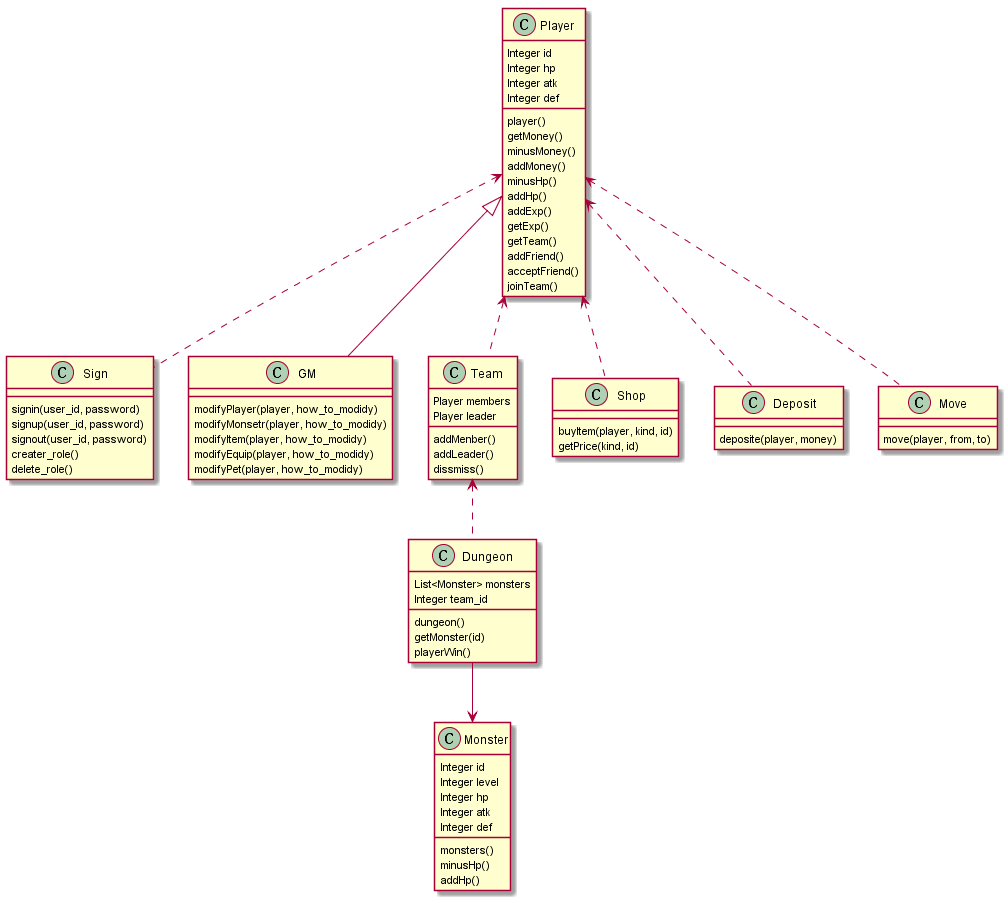
\includegraphics[keepaspectratio=true,width=\dimwidth{1.00}]{./img/10}{}\mdline{446}%mdk

%mdk-data-line={447}
\mdhr{}%mdk

%mdk-data-line={448}
\noindent\mdline{448}\mdcaption{\textbf{Figure~\mdcaptionlabel{11}.}~\mdcaptiontext{模块类图}}%mdk
%mdk
\end{mdcenter}%mdk
\end{figure}%mdk

%mdk-data-line={449}
\subsection{\mdline{449}5.1.\hspace*{0.5em}\mdline{449}登陆模块}\label{51}%mdk%mdk

%mdk-data-line={451}
\noindent\mdline{451}玩家登陆,创建和删除角色。%mdk

%mdk-data-line={453}
\mdline{453}主要函数:%mdk

%mdk-data-line={455}
\begin{itemize}[noitemsep,topsep=\mdcompacttopsep]%mdk

%mdk-data-line={455}
\item\mdline{455}\mdcode{signin(user\_id,~password)}\mdline{455}在数据库中验证参数是否对应%mdk

%mdk-data-line={456}
\item\mdline{456}\mdcode{signup(user\_id,~password)}\mdline{456}在数据库中插入新的用户%mdk

%mdk-data-line={457}
\item\mdline{457}\mdcode{signout(user\_id,~password)}\mdline{457}在后端删除相应的类和session%mdk

%mdk-data-line={458}
\item\mdline{458}\mdcode{creater\_role()}\mdline{458}从数据库中创建角色。%mdk

%mdk-data-line={459}
\item\mdline{459}\mdcode{delete\_role()}\mdline{459}从数据库中删除角色。%mdk
%mdk
\end{itemize}%mdk

%mdk-data-line={461}
\subsection{\mdline{461}5.2.\hspace*{0.5em}\mdline{461}玩家模块}\label{52}%mdk%mdk

%mdk-data-line={463}
\noindent\mdline{463}实现登陆的玩家管理,在攻打副本,购买等操作。%mdk

%mdk-data-line={465}
\mdline{465}主要函数:%mdk

%mdk-data-line={467}
\begin{itemize}[noitemsep,topsep=\mdcompacttopsep]%mdk

%mdk-data-line={467}
\item\mdline{467}\mdcode{player()}\mdline{467}构造函数,初始化登陆的玩家,从数据库中读出玩家基本信息。%mdk

%mdk-data-line={468}
\item\mdline{468}\mdcode{getMoney()}\mdline{468}从数据库中读出玩家的金钱。%mdk

%mdk-data-line={469}
\item\mdline{469}\mdcode{minusMoney()}\mdline{469}从数据库中减去一定数量的金钱。%mdk

%mdk-data-line={470}
\item\mdline{470}\mdcode{addMoney()}\mdline{470}在数据库中增加一定数量的金钱。%mdk

%mdk-data-line={471}
\item\mdline{471}\mdcode{minusHp()}\mdline{471}减少生命值。%mdk

%mdk-data-line={472}
\item\mdline{472}\mdcode{addHp()}\mdline{472}增加生命值。%mdk

%mdk-data-line={473}
\item\mdline{473}\mdcode{addExp()}\mdline{473}在数据库中增加一定数量的经验。%mdk

%mdk-data-line={474}
\item\mdline{474}\mdcode{getExp()}\mdline{474}从数据库中查询玩家的经验。%mdk

%mdk-data-line={475}
\item\mdline{475}\mdcode{getTeam()}\mdline{475}从数据库读取玩家在哪个小队。%mdk

%mdk-data-line={476}
\item\mdline{476}\mdcode{addFriend()}\mdline{476}发出一个好友请求。%mdk

%mdk-data-line={477}
\item\mdline{477}\mdcode{acceptFriend()}\mdline{477}接受好友请求,写入数据库。%mdk

%mdk-data-line={478}
\item\mdline{478}\mdcode{joinTeam()}\mdline{478}加入一个小队,写记录到数据库。%mdk
%mdk
\end{itemize}%mdk

%mdk-data-line={480}
\noindent\mdline{480}主要成员变量:%mdk

%mdk-data-line={482}
\begin{itemize}[noitemsep,topsep=\mdcompacttopsep]%mdk

%mdk-data-line={482}
\item\mdline{482}\mdcode{id}\mdline{482}玩家id。%mdk

%mdk-data-line={483}
\item\mdline{483}\mdcode{hp}\mdline{483}玩家当前生命值。%mdk

%mdk-data-line={484}
\item\mdline{484}\mdcode{atk}\mdline{484}玩家当前攻击力。%mdk

%mdk-data-line={485}
\item\mdline{485}\mdcode{def}\mdline{485}玩家当前防御力。%mdk
%mdk
\end{itemize}%mdk

%mdk-data-line={487}
\subsection{\mdline{487}5.3.\hspace*{0.5em}\mdline{487}管理员模块}\label{53}%mdk%mdk

%mdk-data-line={489}
\noindent\mdline{489}管理员继承了玩家的所有属性。可以参加游戏,可以管理游戏。%mdk

%mdk-data-line={491}
\mdline{491}主要函数:%mdk

%mdk-data-line={493}
\begin{itemize}[noitemsep,topsep=\mdcompacttopsep]%mdk

%mdk-data-line={493}
\item\mdline{493}\mdcode{modifyPlayer(player,~how\_to\_modidy)}\mdline{493}修改玩家相关的数据。%mdk

%mdk-data-line={494}
\item\mdline{494}\mdcode{modifyMonsetr(player,~how\_to\_modidy)}\mdline{494}修改怪物相关的数据。%mdk

%mdk-data-line={495}
\item\mdline{495}\mdcode{modifyItem(player,~how\_to\_modidy)}\mdline{495}修改道具相关的数据。%mdk

%mdk-data-line={496}
\item\mdline{496}\mdcode{modifyEquip(player,~how\_to\_modidy)}\mdline{496}修改道具相关的数据。%mdk

%mdk-data-line={497}
\item\mdline{497}\mdcode{modifyPet(player,~how\_to\_modidy)}\mdline{497}修改宠物相关的数据。%mdk
%mdk
\end{itemize}%mdk

%mdk-data-line={499}
\subsection{\mdline{499}5.4.\hspace*{0.5em}\mdline{499}队伍模块}\label{54}%mdk%mdk

%mdk-data-line={501}
\noindent\mdline{501}管理组队%mdk

%mdk-data-line={503}
\mdline{503}主要函数:%mdk

%mdk-data-line={505}
\begin{itemize}[noitemsep,topsep=\mdcompacttopsep]%mdk

%mdk-data-line={505}
\item\mdline{505}\mdcode{addMenber()}\mdline{505}添加成员记录到数据库和成员变量。%mdk

%mdk-data-line={506}
\item\mdline{506}\mdcode{addLeader()}\mdline{506}添加队长记录到数据库和成员变量。%mdk

%mdk-data-line={507}
\item\mdline{507}\mdcode{dissmiss()}\mdline{507}队长解散组队。%mdk
%mdk
\end{itemize}%mdk

%mdk-data-line={509}
\noindent\mdline{509}主要成员变量:%mdk

%mdk-data-line={511}
\begin{itemize}[noitemsep,topsep=\mdcompacttopsep]%mdk

%mdk-data-line={511}
\item\mdline{511}\mdcode{members}\mdline{511}队员%mdk

%mdk-data-line={512}
\item\mdline{512}\mdcode{leader}\mdline{512}队长%mdk
%mdk
\end{itemize}%mdk

%mdk-data-line={514}
\subsection{\mdline{514}5.5.\hspace*{0.5em}\mdline{514}购物模块}\label{55}%mdk%mdk

%mdk-data-line={516}
\noindent\mdline{516}用于玩家购买道具/宠物/装备。%mdk

%mdk-data-line={518}
\mdline{518}主要函数:%mdk

%mdk-data-line={520}
\begin{itemize}[noitemsep,topsep=\mdcompacttopsep]%mdk

%mdk-data-line={520}
\item\mdline{520}\mdcode{buyItem(player,~kind,~id)}\mdline{520}购买道具/宠物/装备,执行购买事务。%mdk

%mdk-data-line={521}
\item\mdline{521}\mdcode{getPrice(kind,~id)}\mdline{521}获取道具/宠物/装备的价格。%mdk
%mdk
\end{itemize}%mdk

%mdk-data-line={523}
\subsection{\mdline{523}5.6.\hspace*{0.5em}\mdline{523}怪物模块}\label{55.5}%mdk%mdk

%mdk-data-line={525}
\noindent\mdline{525}用于实现游戏中攻打副本时的怪物管理。%mdk

%mdk-data-line={527}
\mdline{527}主要函数:%mdk

%mdk-data-line={529}
\begin{itemize}[noitemsep,topsep=\mdcompacttopsep]%mdk

%mdk-data-line={529}
\item\mdline{529}\mdcode{monsters()}\mdline{529}构造函数,初始化副本产生的怪物,从数据库中读出怪物基本信息。%mdk

%mdk-data-line={530}
\item\mdline{530}\mdcode{minusHp()}\mdline{530}减少生命值。%mdk

%mdk-data-line={531}
\item\mdline{531}\mdcode{addHp()}\mdline{531}增加生命值。%mdk
%mdk
\end{itemize}%mdk

%mdk-data-line={533}
\noindent\mdline{533}主要成员变量:%mdk

%mdk-data-line={535}
\begin{itemize}[noitemsep,topsep=\mdcompacttopsep]%mdk

%mdk-data-line={535}
\item\mdline{535}\mdcode{id}\mdline{535}怪物id。%mdk

%mdk-data-line={536}
\item\mdline{536}\mdcode{level}\mdline{536}怪物等级。%mdk

%mdk-data-line={537}
\item\mdline{537}\mdcode{hp}\mdline{537}怪物当前生命值。%mdk

%mdk-data-line={538}
\item\mdline{538}\mdcode{atk}\mdline{538}怪物当前攻击力。%mdk

%mdk-data-line={539}
\item\mdline{539}\mdcode{def}\mdline{539}怪物当前防御力。%mdk
%mdk
\end{itemize}%mdk

%mdk-data-line={541}
\subsection{\mdline{541}5.7.\hspace*{0.5em}\mdline{541}副本模块}\label{56}%mdk%mdk

%mdk-data-line={543}
\noindent\mdline{543}副本模块管理一次队伍攻打副本的全部内容,包括怪物和队伍。在攻打副本时初始化成员变量。%mdk

%mdk-data-line={545}
\mdline{545}主要函数:%mdk

%mdk-data-line={547}
\begin{itemize}[noitemsep,topsep=\mdcompacttopsep]%mdk

%mdk-data-line={547}
\item\mdline{547}\mdcode{dungeon()}\mdline{547}初始化所有的怪物和他的位置,分配id;生成对战记录写入数据库。%mdk

%mdk-data-line={548}
\item\mdline{548}\mdcode{getMonster(id)}\mdline{548}获取某一个怪物。%mdk

%mdk-data-line={549}
\item\mdline{549}\mdcode{playerWin()}\mdline{549}玩家胜利,写记录%mdk
%mdk
\end{itemize}%mdk

%mdk-data-line={551}
\noindent\mdline{551}主要成员变量:%mdk

%mdk-data-line={553}
\begin{itemize}[noitemsep,topsep=\mdcompacttopsep]%mdk

%mdk-data-line={553}
\item\mdline{553}\mdcode{monsters}\mdline{553}副本中的怪物。%mdk

%mdk-data-line={554}
\item\mdline{554}\mdcode{team\_id}\mdline{554}对战的队伍。%mdk
%mdk
\end{itemize}%mdk

%mdk-data-line={556}
\subsection{\mdline{556}5.8.\hspace*{0.5em}\mdline{556}充值模块}\label{57}%mdk%mdk

%mdk-data-line={558}
\noindent\mdline{558}此模块本因有第三方接口,在作业中简化。%mdk

%mdk-data-line={560}
\mdline{560}主要函数:%mdk

%mdk-data-line={562}
\mdline{562}\mdcode{deposite(player,~money)}\mdline{562}执行充值事务。%mdk

%mdk-data-line={564}
\subsection{\mdline{564}5.9.\hspace*{0.5em}\mdline{564}物品迁移模块}\label{58}%mdk%mdk

%mdk-data-line={566}
\noindent\mdline{566}用于玩家的物品(道具,装备)在仓库、背包等容器中相互迁移。%mdk

%mdk-data-line={568}
\mdline{568}主要函数:%mdk

%mdk-data-line={570}
\mdline{570}\mdcode{move(player,~from,~to)}\mdline{570}执行迁移事务。%mdk

%mdk-data-line={572}
\subsection{\mdline{572}5.10.\hspace*{0.5em}\mdline{572}视图模块}\label{59}%mdk%mdk

%mdk-data-line={574}
\noindent\mdline{574}视图模块负责与用户界面及交互有关的操作。%mdk

%mdk-data-line={576}
\begin{itemize}[noitemsep,topsep=\mdcompacttopsep]%mdk

%mdk-data-line={576}
\item\mdline{576}\mdcode{navigate(direction)}\mdline{576} 向 \mdline{576}\mdcode{dir}\mdline{576} 方向移动角色一格%mdk

%mdk-data-line={577}
\item\mdline{577}\mdcode{open\_menu(menu\_name)}\mdline{577} 打开某个菜单%mdk
%mdk
\end{itemize}%mdk

%mdk-data-line={579}
\noindent\mdline{579}主要成员变量:%mdk

%mdk-data-line={581}
\begin{itemize}[noitemsep,topsep=\mdcompacttopsep]%mdk

%mdk-data-line={581}
\item\mdline{581}\mdcode{stat}\mdline{581} 视图当前所处状态(主世界、副本、菜单等)%mdk

%mdk-data-line={582}
\item\mdline{582}\mdcode{position}\mdline{582} 当前角色所在位置%mdk
%mdk
\end{itemize}%mdk

%mdk-data-line={584}
\begin{figure}[tbp]%mdk
\begin{mdcenter}%mdk

%mdk-data-line={585}
\noindent\mdline{585}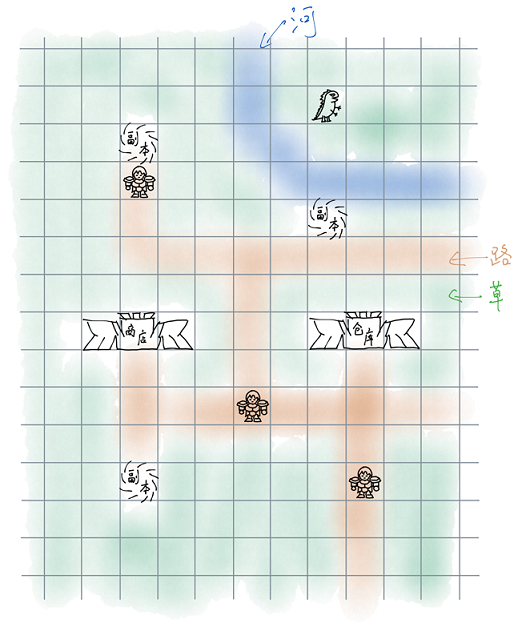
\includegraphics[keepaspectratio=true,width=\dimwidth{0.70}]{./img/UI}{}\mdline{585}%mdk

%mdk-data-line={586}
\mdhr{}%mdk

%mdk-data-line={587}
\noindent\mdline{587}\mdcaption{\textbf{Figure~\mdcaptionlabel{12}.}~\mdcaptiontext{用户界面草图}}%mdk
%mdk
\end{mdcenter}%mdk
\end{figure}%mdk

%mdk-data-line={588}
\section{\mdline{588}6.\hspace*{0.5em}\mdline{588}技术和环境分析}\label{6}%mdk%mdk

%mdk-data-line={590}
\subsection{\mdline{590}6.1.\hspace*{0.5em}\mdline{590}开发技术}\label{61}%mdk%mdk

%mdk-data-line={592}
\begin{itemize}[noitemsep,topsep=\mdcompacttopsep]%mdk

%mdk-data-line={592}
\item\mdline{592}前端

%mdk-data-line={593}
\begin{itemize}[noitemsep,topsep=\mdcompacttopsep]%mdk

%mdk-data-line={593}
\item\mdline{593}HTML%mdk

%mdk-data-line={594}
\item\mdline{594}CSS%mdk

%mdk-data-line={595}
\item\mdline{595}JS (Vue.js)%mdk
%mdk
\end{itemize}%mdk%mdk

%mdk-data-line={596}
\item\mdline{596}后端

%mdk-data-line={597}
\begin{itemize}[noitemsep,topsep=\mdcompacttopsep]%mdk

%mdk-data-line={597}
\item\mdline{597}Web服务器: uWSGI%mdk

%mdk-data-line={598}
\item\mdline{598}Web应用: Django 2.1.4%mdk
%mdk
\end{itemize}%mdk%mdk
%mdk
\end{itemize}%mdk

%mdk-data-line={600}
\subsection{\mdline{600}6.2.\hspace*{0.5em}\mdline{600}开发环境}\label{62}%mdk%mdk

%mdk-data-line={602}
\noindent\mdline{602}Windows 10%mdk

%mdk-data-line={604}
\subsection{\mdline{604}6.3.\hspace*{0.5em}\mdline{604}生产环境}\label{63}%mdk%mdk

%mdk-data-line={606}
\begin{itemize}[noitemsep,topsep=\mdcompacttopsep]%mdk

%mdk-data-line={606}
\item\mdline{606}阿里云服务器 CentOS 7.4%mdk

%mdk-data-line={607}
\item\mdline{607}CPU :1核 Xeon E5%mdk

%mdk-data-line={608}
\item\mdline{608}硬盘:40G SSD%mdk

%mdk-data-line={609}
\item\mdline{609}内存:2G%mdk
%mdk
\end{itemize}%mdk%mdk


\end{document}
